\documentclass[11pt]{article}
\usepackage{euscript}

\usepackage{amsmath}
\usepackage{amsthm}
\usepackage{amssymb}
\usepackage{epsfig}
\usepackage{xspace}
\usepackage{color}
\usepackage{url}

%%%%%%%%%%%%%%%%%%%%%%%%%%%%%%%%%
\setlength{\textheight}{9in}
\setlength{\topmargin}{-0.600in}
\setlength{\headheight}{0.2in}
\setlength{\headsep}{0.250in}
\setlength{\footskip}{0.5in}
\flushbottom
\setlength{\textwidth}{6.5in}
\setlength{\oddsidemargin}{0in}
\setlength{\evensidemargin}{0in}
\setlength{\columnsep}{2pc}
\setlength{\parindent}{1em}
%%%%%%%%%%%%%%%%%%%%%%%%%%%%%%%%%


\newcommand{\eps}{\varepsilon}

\renewcommand{\c}[1]{\ensuremath{\EuScript{#1}}}
\renewcommand{\b}[1]{\ensuremath{\mathbb{#1}}}
\newcommand{\s}[1]{\textsf{#1}}

\newcommand{\E}{\textbf{\textsf{E}}}
\renewcommand{\Pr}{\textbf{\textsf{Pr}}}

\title{Homework 3 Data Mining
\footnote{\s{CS 6955 Data Mining; \;\; Spring 2012 \hfill
Instructor: Jeff M. Phillips, University of Utah}
}
}
\author{Alex Clemmer}

\begin{document}
\maketitle





%%%%%%%%%%%%%%%%%%%%%%%%%%%%%%%%%%%%%%%%%%%%%%%%%%%%
%%%%%%%%%%%%%%%%%%%%%%%%%%%%%%%%%%%%%%%%%%%%%%%%%%%%
%%%%%%%%%%%%%%%%%%%%%%%%%%%%%%%%%%%%%%%%%%%%%%%%%%%%

\section{Shingling}

\paragraph*{A:} The breakdown of shingles is as follows:

\begin{center}

\begin{tabular}{| c || c | c | c | c |}
\hline
& \textbf{D1.txt} & \textbf{D2.txt}  & \textbf{D3.txt}  & \textbf{D4.txt} \\
\hline
\hline
$k = 5$ & 4217 & 3679 & 2589 & 1418 \\
\hline
8 & 5821 & 5089 & 3301 & 1722 \\
\hline
4 & 1133 & 1012 & 622 & 300 \\
\hline

\end{tabular}

\end{center}


\paragraph*{B:} The Jaccard coefficient for each pair of documents is as follows:

\begin{center}

\begin{tabular}{| c || c | c | c | c |}
\hline
\multicolumn{5}{|c|}{$5$-character} \\
\hline
& \textbf{D1.txt} & \textbf{D2.txt}  & \textbf{D3.txt}  & \textbf{D4.txt} \\
\hline
\hline
\textbf{D1.txt} &  & 0.179740 & 0.170220 & 0.082613 \\
\hline
\textbf{D2.txt} &  & & 0.146306 & 0.081706 \\
\hline
\textbf{D3.txt} &  &  &  & 0.069104 \\
\hline
\textbf{D4.txt} &  &  &  &  \\
\hline
\end{tabular}

\end{center}

\begin{center}

\begin{tabular}{| c || c | c | c | c |}
\hline
\multicolumn{5}{|c|}{$8$-character} \\
\hline
& \textbf{D1.txt} & \textbf{D2.txt}  & \textbf{D3.txt}  & \textbf{D4.txt} \\
\hline
\hline
\textbf{D1.txt} &  & 0.052682 & 0.053835 & 0.016440 \\
\hline
\textbf{D2.txt} &  & & 0.036442 & 0.016415 \\
\hline
\textbf{D3.txt} &  &  &  & 0.012906 \\
\hline
\textbf{D4.txt} &  &  &  &  \\
\hline
\end{tabular}

\end{center}

\begin{center}

\begin{tabular}{| c || c | c | c | c |}
\hline
\multicolumn{5}{|c|}{$4$-word} \\
\hline
& \textbf{D1.txt} & \textbf{D2.txt}  & \textbf{D3.txt}  & \textbf{D4.txt} \\
\hline
\hline
\textbf{D1.txt} &  & 0.001868 & 0.004579 & 0.000000 \\
\hline
\textbf{D2.txt} &  & & 0.000000 & 0.000000 \\
\hline
\textbf{D3.txt} &  &  &  & 0.000000 \\
\hline
\textbf{D4.txt} &  &  &  &  \\
\hline
\end{tabular}

\end{center}














\section{Min Hashing}

\paragraph{A:} The following results implement the ``stock" hash function supplied in the assignment. The results are patently awful. We rectify this with more experiments in part B.

\begin{center}

\begin{tabular}{| c || c | c | c | c |}
\hline
\multicolumn{5}{|c|}{$t = 10$} \\
\hline
& \textbf{D1.txt} & \textbf{D2.txt}  & \textbf{D3.txt}  & \textbf{D4.txt} \\
\hline
\hline
\textbf{D1.txt} &  & 0.2 & 0.1 & 0 \\
\hline
\textbf{D2.txt} &  & & 0.1 & 0 \\
\hline
\textbf{D3.txt} &  &  &  & 0 \\
\hline
\textbf{D4.txt} &  &  &  &  \\
\hline
\end{tabular}

\end{center}


\begin{center}

\begin{tabular}{| c || c | c | c | c |}
\hline
\multicolumn{5}{|c|}{$t = 50$} \\
\hline
& \textbf{D1.txt} & \textbf{D2.txt}  & \textbf{D3.txt}  & \textbf{D4.txt} \\
\hline
\hline
\textbf{D1.txt} &  & 0.06 & 0.08 & 0 \\
\hline
\textbf{D2.txt} &  & & 0.02 & 0 \\
\hline
\textbf{D3.txt} &  &  &  & 0 \\
\hline
\textbf{D4.txt} &  &  &  &  \\
\hline
\end{tabular}

\end{center}


\begin{center}

\begin{tabular}{| c || c | c | c | c |}
\hline
\multicolumn{5}{|c|}{$t = 100$} \\
\hline
& \textbf{D1.txt} & \textbf{D2.txt}  & \textbf{D3.txt}  & \textbf{D4.txt} \\
\hline
\hline
\textbf{D1.txt} &  & 0.04 & 0.07 & 0.01 \\
\hline
\textbf{D2.txt} &  & & 0.02 & 0.01 \\
\hline
\textbf{D3.txt} &  &  &  & 0 \\
\hline
\textbf{D4.txt} &  &  &  &  \\
\hline
\end{tabular}

\end{center}


\begin{center}

\begin{tabular}{| c || c | c | c | c |}
\hline
\multicolumn{5}{|c|}{$t = 300$} \\
\hline
& \textbf{D1.txt} & \textbf{D2.txt}  & \textbf{D3.txt}  & \textbf{D4.txt} \\
\hline
\hline
\textbf{D1.txt} &  & 0.06 & 0.076666 & 0.02 \\
\hline
\textbf{D2.txt} &  & & 0.03 & 0.02 \\
\hline
\textbf{D3.txt} &  &  &  & 0.02 \\
\hline
\textbf{D4.txt} &  &  &  &  \\
\hline
\end{tabular}

\end{center}

\begin{center}

\begin{tabular}{| c || c | c | c | c |}
\hline
\multicolumn{5}{|c|}{$t = 600$} \\
\hline
& \textbf{D1.txt} & \textbf{D2.txt}  & \textbf{D3.txt}  & \textbf{D4.txt} \\
\hline
\hline
\textbf{D1.txt} &  & 0.061666 & 0.0566666 & 0.015 \\
\hline
\textbf{D2.txt} &  & & 0.03 & 0.0183333 \\
\hline
\textbf{D3.txt} &  &  &  & 0.015 \\
\hline
\textbf{D4.txt} &  &  &  &  \\
\hline
\end{tabular}

\end{center}



\paragraph{B:} Because of the poor quality of these results, I chose to also implement another family of hash functions. Basically, we generate a random string, supplement it with the row number $r$, and run MD5 on that, modding this number by $m$. The results are in the tables that follow.

The MD5 method is orders of magnitude slower than the really bad hash function. It took minutes to run, versus the bad hash's instantaneous results. The results are much better, but obviously the time tradeoff is precipitous. The advantage is that it is ``embarrassingly parallel".





\begin{center}

\begin{tabular}{| c || c | c | c | c |}
\hline
\multicolumn{5}{|c|}{$t = 10$} \\
\hline
& \textbf{D1.txt} & \textbf{D2.txt}  & \textbf{D3.txt}  & \textbf{D4.txt} \\
\hline
\hline
\textbf{D1.txt} &  & 0.0 & 0.0 & 0.1 \\
\hline
\textbf{D2.txt} &  & & 0.1 & 0.1 \\
\hline
\textbf{D3.txt} &  &  &  & 0.0 \\
\hline
\textbf{D4.txt} &  &  &  &  \\
\hline
\end{tabular}

\end{center}


\begin{center}

\begin{tabular}{| c || c | c | c | c |}
\hline
\multicolumn{5}{|c|}{$t = 50$} \\
\hline
& \textbf{D1.txt} & \textbf{D2.txt}  & \textbf{D3.txt}  & \textbf{D4.txt} \\
\hline
\hline
\textbf{D1.txt} &  & 0.1 & 0.1 & 0.04 \\
\hline
\textbf{D2.txt} &  & & 0.06 & 0.04 \\
\hline
\textbf{D3.txt} &  &  &  & 0.02 \\
\hline
\textbf{D4.txt} &  &  &  &  \\
\hline
\end{tabular}

\end{center}


\begin{center}

\begin{tabular}{| c || c | c | c | c |}
\hline
\multicolumn{5}{|c|}{$t = 100$} \\
\hline
& \textbf{D1.txt} & \textbf{D2.txt}  & \textbf{D3.txt}  & \textbf{D4.txt} \\
\hline
\hline
\textbf{D1.txt} &  & 0.07 & 0.1 & 0.03 \\
\hline
\textbf{D2.txt} &  & & 0.08 & 0.04 \\
\hline
\textbf{D3.txt} &  &  &  & 0.4 \\
\hline
\textbf{D4.txt} &  &  &  &  \\
\hline
\end{tabular}

\end{center}


\begin{center}

\begin{tabular}{| c || c | c | c | c |}
\hline
\multicolumn{5}{|c|}{$t = 300$} \\
\hline
& \textbf{D1.txt} & \textbf{D2.txt}  & \textbf{D3.txt}  & \textbf{D4.txt} \\
\hline
\hline
\textbf{D1.txt} &  & 0.1166 & 0.10333 & 0.023333 \\
\hline
\textbf{D2.txt} &  & & 0.08 & 0.036666 \\
\hline
\textbf{D3.txt} &  &  &  & 0.026666 \\
\hline
\textbf{D4.txt} &  &  &  &  \\
\hline
\end{tabular}

\end{center}

\begin{center}

\begin{tabular}{| c || c | c | c | c |}
\hline
\multicolumn{5}{|c|}{$t = 600$} \\
\hline
& \textbf{D1.txt} & \textbf{D2.txt}  & \textbf{D3.txt}  & \textbf{D4.txt} \\
\hline
\hline
\textbf{D1.txt} &  & 0.12333 & 0.10333 & 0.023333 \\
\hline
\textbf{D2.txt} &  & & 0.08 & 0.036666 \\
\hline
\textbf{D3.txt} &  &  &  & 0.028888 \\
\hline
\textbf{D4.txt} &  &  &  &  \\
\hline
\end{tabular}

\end{center}



\section{LSH}

\paragraph*{A:} There is arguably not a tremendously good fit, but empirically it works out that when $r = 4, b = 25$ ends up being the best. Note that this optimizes specifically for false positive, but this is a consequence of the equation supplied. It is trivial to run the same experiment for false negatives, but we didn't because the assignment did not seem to ask for it.

\begin{center}
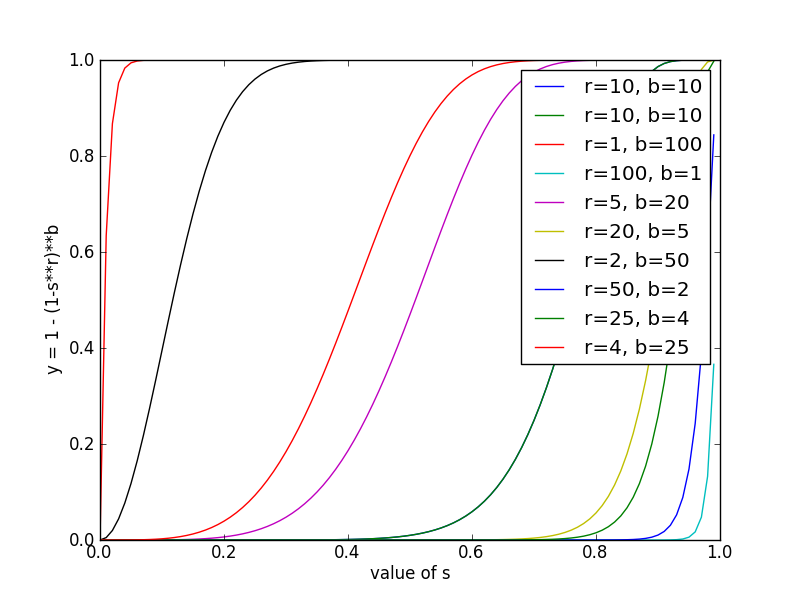
\includegraphics[scale=0.5]{plot.png}
\end{center}

\paragraph*{B:} Because the documents are not very similar according to our minhashing scheme, these probabilities will be pretty small. Given our estimating function $S(\cdot)$, then for some probability $q$, we determine this as $S(q)$. The results follow.

\begin{center}

\begin{tabular}{| c || c | c | c | c |}
\hline
\multicolumn{5}{|c|}{$8$-character} \\
\hline
& \textbf{D1.txt} & \textbf{D2.txt}  & \textbf{D3.txt}  & \textbf{D4.txt} \\
\hline
\hline
\textbf{D1.txt} &  & 0.000193 & 0.00021 & 0.000002 \\
\hline
\textbf{D2.txt} &  & & 0.000044 & 0.000002 \\
\hline
\textbf{D3.txt} &  &  &  & $6.93596 \cdot 10^{-7}$ \\
\hline
\textbf{D4.txt} &  &  &  &  \\
\hline
\end{tabular}

\end{center}






\end{document}
